\documentclass[11pt,a4paper]{article}

\usepackage[utf8]{inputenc}
\usepackage[spanish,mexico]{babel}

\usepackage{amsmath, amssymb, amsthm}
\usepackage{mathrsfs}
\usepackage{appendix}

\usepackage{hyperref}
\usepackage{captdef}

\usepackage{psfrag}
\usepackage{graphicx}
%\usepackage{subfig}
\usepackage{color}
\usepackage{multicol} 

%\usepackage{fancyhdr}
%\pagestyle{fancy}
%\fancyhf{}


\usepackage{cancel}
\usepackage[usenames,dvipsnames,svgnames,table]{xcolor}
\usepackage[left=2cm,right=2cm,top=2cm,bottom=2cm]{geometry}
\usepackage{caption}
\usepackage{subcaption}
%\renewcommand{\baselinestretch}{1.5}

\usepackage{hyperref}
%\usepackage[hidelinks]{hyperref} 
\hypersetup{
    colorlinks=true,
    linkcolor=blue,
    filecolor=magenta,      
    urlcolor=cyan,
    }

\begin{document}
\thispagestyle{empty}

\includegraphics[height=3.5cm]{escudoCiencias.pdf}
\vspace{-3.8cm}
\begin{flushright}
\hspace{4cm}
{\Large\textbf{Borrador de Tesis}\\
Para ser Físico}
\vspace{0.3cm}\\
\begin{large}Autor: Rodrigo Vega Vilchis.\end{large}\\
\begin{footnotesize}
Correo: rockdrigo6@ciencias.unam.mx\\
\hspace{2.05cm}{\color{white}.}\\
\end{footnotesize}
\vspace{0.75cm}

\end{flushright}
%\vspace{.4cm}
 \hrule height1pt\vspace{.5cm}


\section{Introducción}

%Tenemos que enfocarnos en Marco Teórico en general, Hipótesis, objetivos y limites y alcances de la tesis.

Nuestra curiosidad como seres humanos ha sido el motor para el planteamiento de las grandes preguntas que nos abrieron camino hasta nuestra época y todo lo que conocemos de ella. La fenomenología de nuestro mundo fue (y es) tan impactante que captó la atención de los antigüos pensadores y pusieron en marcha reflexiones sobre cómo percibían el mundo; y con el tiempo fueron construyendo peldaño tras peldaño: las teorías que rigen la naturaleza. Las preguntas más influyentes que puedo rescatar para la construcción del futuro, fueron acerca del cambio de las cosas y el lugar que ocupamos en el universo.

De acuerdo a la cosmogonía de una gran variedad de culturas alrededor del mundo, coinciden que todo ha emergido del caos y que fueron algunas fuerzas superiores las que generaron el orden para darnos vida a todo lo que conocemos; ya desde un principio se tuvo una íntima relación con el \emph{caos} como parte natural de la vida y para poder llegar a entenderlo tuvieron que pasar toda una serie de acontecimientos de los cuales nunca terminaríamos de mencionarlos a todos. Es posible resaltar algunos de ellos, de los cuales fueron el centro de ideas que se fueron desarrollando hasta la culminación de lo que buscamos. Hacia los inicios de la cultura griega existieron dos grandes planteamientos sobre el cambio y la inmovilidad, dados por Heráclito y Parménides\footnote{Propone la inmovilidad como una ley. Su demostración recae en el ser, afirmando que siempre será, pues si cambia hacia el ser el resultado es que no cambia y si cambia al no-ser llegaríamos a una contradicción, pues es imposible su existencia. El desarrollo de la ciencia actual nos insinua una relación con la conservación de la energía, pues al final somos solo una única expresión de ella.} respectivamente. 

Heráclito proponía que la secuencia de las experiencias hace que todo cambie por el irremediable paso del tiempo, el hombre que alguna vez estuvo en el río, no será el mismo hombre cuando lo visite de nuevo ni el río el mismo río. Bajo esta bella proposición se puede percibir entre lineas: la presencia de la dinámica\footnote{Que tendría su nacimiento hasta la hazaña de Newton.}, que  la definimos como el cambio de estado de cualquier sistema. Para entonces, sin querer ya se estaban sentando las bases de uno de los grandes ejes de la ciencia, pues en épocas venideras los esfuerzos se concentraron en tratar de modelar el cambio a partir de sus variables.

El siguiente acontecimiento que considero clave y como punto de partida para desarrollar las ideas de la dinámica tuvo que ver con la cosmovisión del universo que nos tocó ¿Como se mueve nuestra bóveda celeste? y ¿En dónde nos encontramos? Hacia finales de la cultura griega encontramos por primera vez a Aristarco de Samos quien propuso el primer modelo heliocentrista, por desgracia casi no quedan registros de su trabajo; no obstante las ideas del geocentrismo fueron las más aceptadas y sostenidas incluso por Aristóteles\footnote{El análogo a Newton de los griegos.}. Claudio Ptolomeo fue quien con sus observaciones y cálculos terminó por establecer el geocentrismo como modelo planetario y así se sostuvo por ¡catorce siglos!

El hito de \emph{Sobre las revoluciones de las orbes celestes} marcó el primer antecedente del regreso a la visión heliocentrista. Pero tuvieron que pasar otros doscientos años para que terminase por ser aceptada y reconocida. La gran labor fue culminada por Sir Isaac Newton con sus tres tomos de \emph{Principios matemáticos de la filosofía natural.} En donde se encarga de introducir axiomas, teoremas, demostraciones, inventar el cálculo con el nombre de \emph{fluxiones}, invalidar la teoría de los vórtices de Descartes, plasmar sus tres leyes que fundamentan toda la dinámica lineal y al final proponer una teoría completa de la dinámica celeste: la gravitación universal. 

Este momento histórico ha sido el cenit de los planteamientos del cambio de Heráclito; la \emph{dinámica} por fin ha sido creada, y con ella las ecuaciones diferenciales (lineales) que la modelan. Con el problema de los dos cuerpos resuelto, una gran cantidad de sistemas modelados, teorías emergentes a partir de los principios de la dinámica, una notoria evolución matemática para el tratamiendo de sistemas cada vez más complejos y demás, se creyó que se había llegado al cenit de los descubrimientos al punto de creer en un \emph{determinismo}; dadas las condiciones iniciales de algún suceso, con las herramientas de la dinámica podríamos predecir cualquier movimiento, hasta que llegó el problema de los tres cuerpos.

Este problema se planteó como reto y al que ganara se le entregaría un premio y reconocimiento, se creyó que era una extensión del trabajo de Newton y que podría darse directo pero en realidad enfrentaron a un problema muy riguroso que no tiene solución analítica. Esto nos hace preguntarnos ¿por qué el anexo de un cuerpo más al baile celeste implicaría una rotunda complejidad? la respuesta recae en la interacciones, pero ya llegarmos a ello. A finales del siglo XVIII, Henri Poincaré fue el dichoso de resolver el problema bajo una perspectiva distinta a la de “predecir'' las posiciones de los astros participantes. Su razonamiento consistía en preguntarse sobre la estabilidad del sistema, si estabamos frente a un sistema estable o eventualmente los astros podrían salirse de órbita y escapar hacia la nada.

Esta nueva perspectiva dio una nueva forma de ver a la dinámica, pues en su trabajo consiguío los primeros descubrimientos de lo que es el \emph{caos}, entendiéndolo como la sensibilidad del sistema a pequeñas perturbaciones en las condiciones iniciales, resultando en comportamientos aperiódicos e impredecibles a largo plazo, aún cuando se tratase de un sistema determinista. Para ponerlo en perspectiva pensemos que la mecánica cuántica trabaja con una función de onda que se rige por distribuciones de probabilidad, las cantidades que se computan no pueden predecirse porque se encuentran indeterminadas, lo único que podemos es estimar la probabilidad con la que podríamos encontrarlas; sin embargo en este caso hablamos de sistemas no deterministas. El caos presenta la misma conjetura de impredictibilidad de las cantidades presentes solamente que para sistemas deterministas, y la gran pregunta es ¿por qué? o ¿qué sistemas presentan caos y cuales no?

Entrando el siglo XX se llevaron a cabo revoluciones científicas en torno al entendimiento de la dinámica, tanto la mecánica cuántica y la relatividad fueron las grandes emergencias que surgieron como evolución de la dinámica de Newton, nuevas teorías se construyeron y desarrollaron hasta hoy día. La dinámica no lineal pudo considerarse como la precursora de las anteriores por cuestiones de fecha y posiblemente matemáticas disponibles. 

Entiéndase la dinámica no lineal como una evolución directa de la dinámica de Newton solo que se consideran sistemas en donde intervienen más de dos interacciones, es decir, el cambio de un sistema en donde interaccionan entre sí tres o más variables. El ejemplo principal es el problema de los tres cuerpos, pero en realidad la gran mayoría de situaciones de la vida real se puede modelar con dinámica no lineal, por la cantidad de interacciones. Por el contrario, en la naturaleza es dificil encontrar sistemas lineales, aquellos que los puedes separar en partes y resolverlos; la naturaleza es más compleja y la mayoría de la veces el total es más que la suma de las partes.

Los avances de la dinámica no lineal se vieron reflejadas en cuestiones de ingeniería para la contrucción de láseres, radares y radios; y en la parte teórica el avance fue sobre construcción de matemática más sofisticada para resolver problemas más complejos de la mecánica clásica. Será hasta la década de los 60s con la llegada de las computadoras con capacidad de resolver grandes cantidades de cálculos que Edward Lorenz desarrolló un sistema de ecuaciones diferenciales no lineales acompladas capaz de predecir el clima y entender mejor las dinámicas atmosféricas. Bajo un sutil accidente en donde la máquina dejó de computar resultados, quiso continuarlos con una pequeña pertubación en las condiciones iniciales y el resultado fue una cosa completamente distinta a la que se venía desarrollando.

Con este trabajo, Lorenz había confirmado la sensibilidad a condiciones iniciales de Poincaré y consigo el caos que se esconde por ser un sistema que cuenta con la interacción de tres variables. Así mismo introdujo el concepto de atractores extraños y de ahí se nos vino toda una ola de estudios fuertes en \emph{teoría del caos}. La conclusión del sistema de Lorenz es que nunca llegaría a un punto de equilibrio en donde oscilara en un periodo dado, en lugar de ello se ha encontrado nuevamente con oscilaciones no periódicas e impredecibles para tiempos largos, esta conclusión es la principal premisa de la teoría del caos.

%Bajo estos descubrimientos, la humanidad ha comenzado a definir el caos de manera formal y no como lo que se le conocía antes, como un desorden de objetos y magnitudes que no tienen un sentido definido. El caos se le comprende como un fenómeno que emerge a partir de la interacción de 3 o más individuos y que cuyas interacciones generan hechos impredecibles.

De la dinámica no lineal y la emergente teoría del caos surgieron nuevos trabajos enfocados en dinámica de fluidos específicamente en turbulencia (hasta hoy en día hablar de hidrodinámica es un tema bastante complejo de abordar); también surgieron trabajos en dinámica de poblaciones, cómo crecen e interaccionan las poblaciones de acuerdo a una serie de hipótesis; se realizaron experimentos en reacciones químicas, circuitos eléctrónicos, nuevos tipos de osciladores armónicos, semiconductores e inclusive en oscilaciones no lineales en sistemas biológicos.

Aunque todavía hay una gran serie de áreas en las que han abordado la dinámica y el caos, es importante que el lector aprecie el camino de la ciencia del cambio, la dinámica ya no es una rama más de la física sino que rebasó sus fronteras y ha explorado otros terrenos con otras perspectivas, marcos teóricos e hipótesis. En el presente trabajo se desarrollará una aplicación de la dinámica bajo la perspectiva ecológica de la interacción entre poblaciones.

Una población esta compuesta por un gran número de individuos, podemos constatar de que todos ellos comparten características de forma que los podamos ver como un sistema homogéneo; si dos poblaciones distintas interactúan bajo ciertas hipótesis, serán interacciones entre individuos de las poblaciones y probablemente entre individuos de su misma especie. Este trabajo analizára cómo son esas interacciones, qué condiciones se necesiten para que el sistema sea estable o inestable y se explorará sobre la existencia de transiciones de fase. Se quiere hallar si en un sistema inmunológico con cáncer existe una transición de cáncer a metástasis bajo las reglas de la dinámica no lineal.

Para ello se van a modelar sistemas computacionales que nos faciliten los cálculos y el entendimiento de las situaciones.




%Su contraparte Parménides propone la inmovilidad como una ley. Su demostración recae en el ser, afirmando que siempre será, pues si cambia hacia el ser el resultado es que no cambia y si cambia al no-ser llegaríamos a una contradicción, pues es imposible su existencia. El desarrollo de la ciencia actual nos insinua una relación con la conservación de la energía, pues al final somos solo una única expresión de ella.



\section{Planteamiento del problema}

%Aquí vamos a introducir el problema de forma más específica. Enfocar todo lo de la introducción en el problema del cancer y lo que se espera. También es importante mencionar los trabajos que estan relacionados a este estudio: los de May, steffano, y el resto de articulos sobre el cancer. 

%Todo lo de la introducción enfocarlo en el proyecto. Hablar de la bibliografía como forma de mostrar los antecedentes del proyecto, de forma cronológica si se puede. Deberá ir primero las fuentes que hablen desde la generalidad y luego las que sean más específicas.

Lo maravilloso del estudio de la física es la simplicidad de sus leyes y teorías, los esfuerzos reunidos hasta ahora han sido capaces de modelar los fenómenos bajo el control de algunas ecuaciones diferenciales ya sean parciales u ordinarias\footnote{En este caso la fenomenología que interviene es lineal, obedecen el principio de superposición.}. No obstante, cuando salimos de este marco de referencia y percibimos el mundo con nuestros sentidos, nos encontramos con diversas estructuras altamente organizadas y complejas tales como: ecosistemas, poblaciones, seres vivos, estructuras ígneas, mercados financieros, etc. Estas estructuras son consideradas como \emph{sistemas complejos} y  las podemos definir como estructuras con variaciones o fluctuaciones constantes\footnote{Esta definición no es absoluta, pues hasta la idea detrás de los sistemas complejos es amplia y valga la redundancia compleja de definir.}.

Estas variaciones las presentan cada una de las partes involucradas del sistema y cada una de ellas puede afectar a otra de forma que el conjunto de sus interacciones sea complejo de determinar e imposibles de predecir, de hecho cuanto más avanza el tiempo son más impredecibles. Por lo tanto, en los sistemas complejos es indiscutible la presencia del \emph{caos}. El caos es una propiedad de los sistemas que presentan más de tres interacciones entre sí; esta propiedad desemboca en dos grandes características: sensibilidad a condiciones iniciales y aperiodicidad del fenómeno que resultan en la impredictibilidad para tiempos largos.


La gran diferencia entre los sistemas físicos y los sistemas complejos recaen en su número de interacciones; mientras que los sistemas físicos pueden separarse en partes porque cumplen el principio de superposición, los sistemas complejos al ser \emph{no lineales}, no pueden separarse en partes. En ese caso las partes y su suma contribuye al todo pero no lo iguala, el todo se convierte en una estructura compleja de la que deviene en caos. El sistema que se estudiará en este trabajo esta enfocado a la dinámica de poblaciones. 

La ecología es la rama de la ciencia que concentra más avances en el área pues su principal misión es la de observar y cuantificar las interacciones de los elementos de un ecosistema, ya sean plantas, seres vivos hervíboros, carnívoros y su relación incluso con el ser humano. En específico nosotros nos centraremos en el crecimiento de las poblaciones y sus interacciones con otras. Para ello vamos a comenzar  introduciendo el primer modelo de crecimiento de poblaciones.

Sea cualquier población en crecimiento sin restricciones de espacio y recursos, las cantidades implicadas que tenemos son
\begin{itemize}
\item Tiempo, siendo esta una variable independiente
\item Población, siendo la variable dependiente
\item Constante de proporcionalidad $r$, esta constante nos muestra la tasa de crecimiento de la población.
\end{itemize}
Con estos elementos podemos generar una ecuación que nos muestre la razón de cambio del crecimiento de la población,
\begin{equation}\label{eq:sinLim}
\frac{dP}{dt}=rP
\end{equation}
en palabras significa que la razón de cambio de la población esta dada por la población\footnote{La cantidad de habitantes que la conforman} definida en un cierto tiempo multiplicada por la tasa de crecimiento. El resultado de resolver esta sencilla ecuación diferencial es
$$P(t)=P_0e^{rt}$$
Notemos que para un tiempo cero tenemos una condición inicial $P_0$ que representa la población inicial en cuestión. Como el crecimiento es exponencial, es de esperarse que para $t\to\infty$ la población también tienda e infinito, lo cual es imposible en nuestro mundo ya que normalmente las poblaciones necesitan de espacio y recursos para su crecimiento, y tal es la dependencia de estos principales factores que la población puede crecer o decrecer hasta extinguirse.
\begin{figure}[h!]
\centering
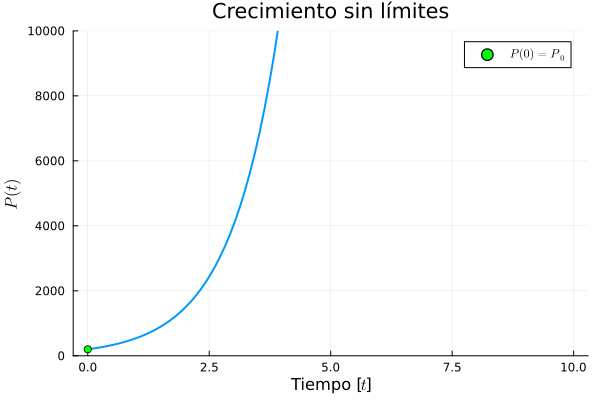
\includegraphics[scale=.5]{Imagenes/Crecimiento sin limites}
\caption{Crecimiento sin límites del resultado de la ecuación \ref{eq:sinLim}.}
\end{figure}

%Siguiente parte: DEfinir la ecuación logística que resuelva este aspecto del modelo anterior, introducir nuevas hipótesis y al final dar un contexto histórico BREVE de la ecuación logística

%Ya de ahí nos vamos recio con LotkaVolterra. Pero quizás haya que hacer un breve mención de sistemas lineales y espacios fase.






\end{document}